\documentclass[11pt]{article}

\usepackage[a4paper,margin=1in]{geometry}
\usepackage{amsmath}
\usepackage{booktabs}
\usepackage{graphicx}
\usepackage{float}

\graphicspath{{report/figures/}{figures/}}

\title{Healthcare Risk Classification Using Logistic Regression and Naive Bayes}
\author{Junior Data Science Portfolio Project}
\date{May 2026}

\begin{document}

\maketitle

\begin{abstract}
This report presents a small healthcare data science project using a medical insurance cost dataset. I define a binary target, \texttt{high\_cost}, by labelling records above the 75th percentile of charges as high cost. I then compare two interpretable probabilistic classifiers: logistic regression and Gaussian Naive Bayes. The project is intended as a mathematically grounded student portfolio piece, with emphasis on probability, odds, coefficient interpretation, Bayes theorem, and classification metrics. This project studies statistical relationships in the dataset and does not prove medical causation.
\end{abstract}

\section{Introduction}

I wanted this project to be simple enough to explain clearly, but still serious enough to show mathematical understanding. The dataset contains medical insurance charges and basic personal attributes such as age, BMI, smoking status, number of children, sex, and region. The question I explored was whether simple interpretable models can classify records into a high-cost group.

This is not a clinical project. Prediction, association, correlation, and causality are different ideas. A model can learn that two variables appear together in this dataset, but that does not mean one medically causes the other. Throughout the report, I treat the results as statistical relationships only.

The implementation uses Python, pandas, matplotlib, and scikit-learn \cite{mckinney2010,pedregosa2011,hunter2007}. I avoided more advanced models because the goal is not to maximise complexity. The goal is to understand the models well enough to defend them.

\section{Dataset and Target Definition}

The dataset has 1,338 rows and the following columns: \texttt{age}, \texttt{sex}, \texttt{bmi}, \texttt{children}, \texttt{smoker}, \texttt{region}, and \texttt{charges}. There are no missing values in the provided CSV file.

The target is constructed as
\[
\texttt{high\_cost} =
\begin{cases}
1, & \text{if charges are above the 75th percentile},\\
0, & \text{otherwise}.
\end{cases}
\]

For this dataset, the 75th percentile is approximately \(\$16,639.91\). I used this threshold because it gives a clear educational definition of a high-cost group and turns a regression-style variable into a classification target. The threshold is still arbitrary. It should not be interpreted as a clinical or policy boundary.

The class balance is shown in Figure~\ref{fig:class-balance}. There are 1,003 records in class 0 and 335 records in class 1, so the target is moderately imbalanced. This is why I report precision, recall, and F1-score as well as accuracy.

\begin{figure}[H]
    \centering
    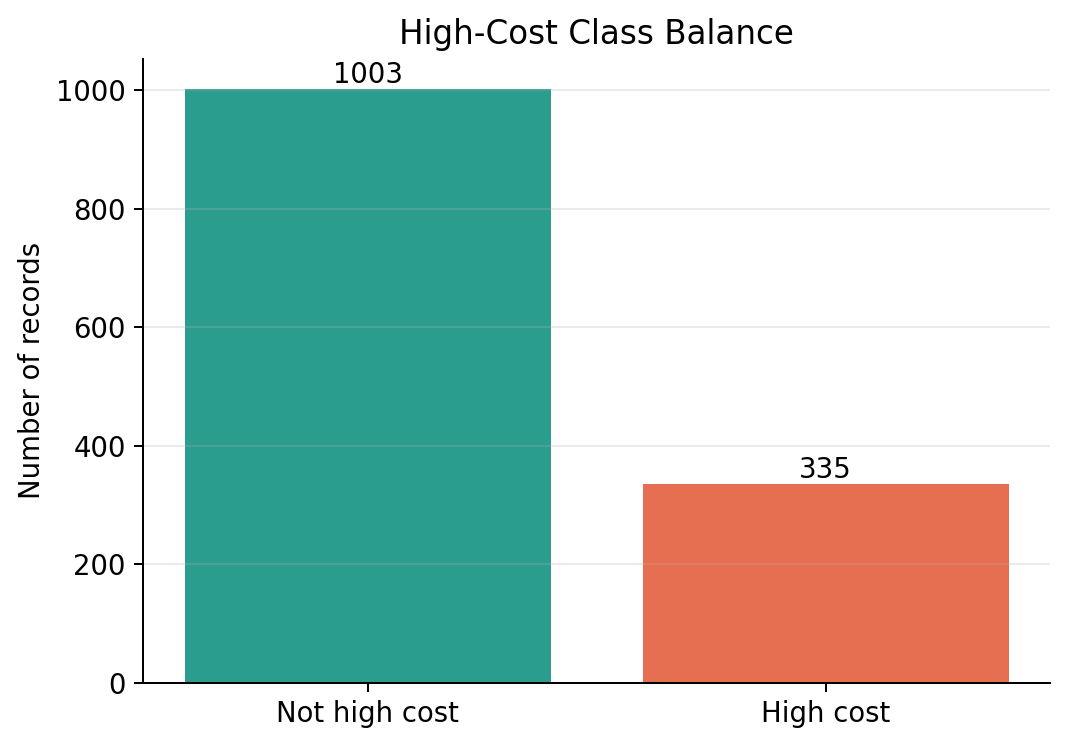
\includegraphics[width=0.68\textwidth]{high_cost_class_balance.png}
    \caption{Class balance for the constructed \texttt{high\_cost} target.}
    \label{fig:class-balance}
\end{figure}

\section{Exploratory Analysis}

Figure~\ref{fig:charges} shows the distribution of charges. The distribution is right-skewed, with many lower-cost records and a smaller number of much higher-cost records. The vertical line marks the 75th percentile threshold used for the target.

\begin{figure}[H]
    \centering
    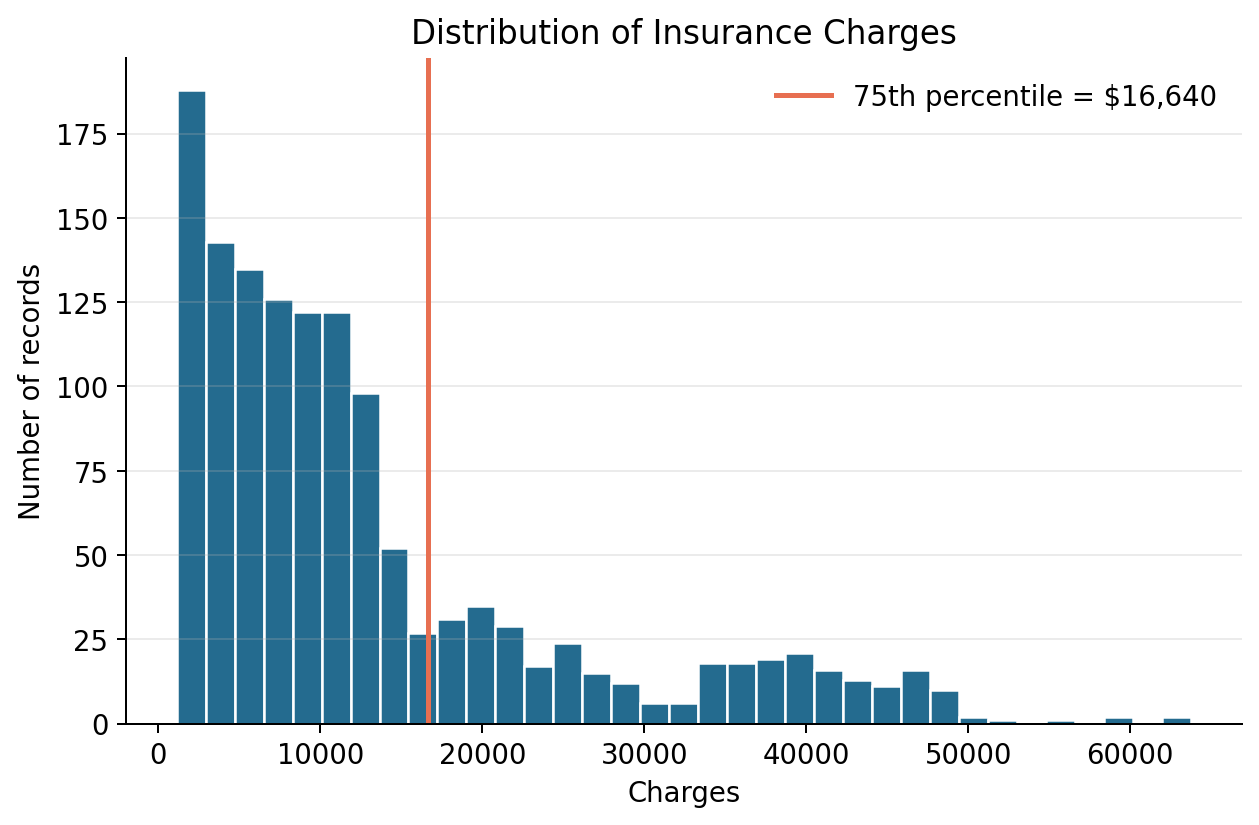
\includegraphics[width=0.82\textwidth]{charges_distribution.png}
    \caption{Distribution of insurance charges with the 75th percentile threshold.}
    \label{fig:charges}
\end{figure}

Because charges are skewed, I also plotted \(\log(\text{charges})\). Figure~\ref{fig:log-charges} shows that the log transformation makes the distribution easier to inspect visually. I did not use log charges as a model feature because charges define the target.

\begin{figure}[H]
    \centering
    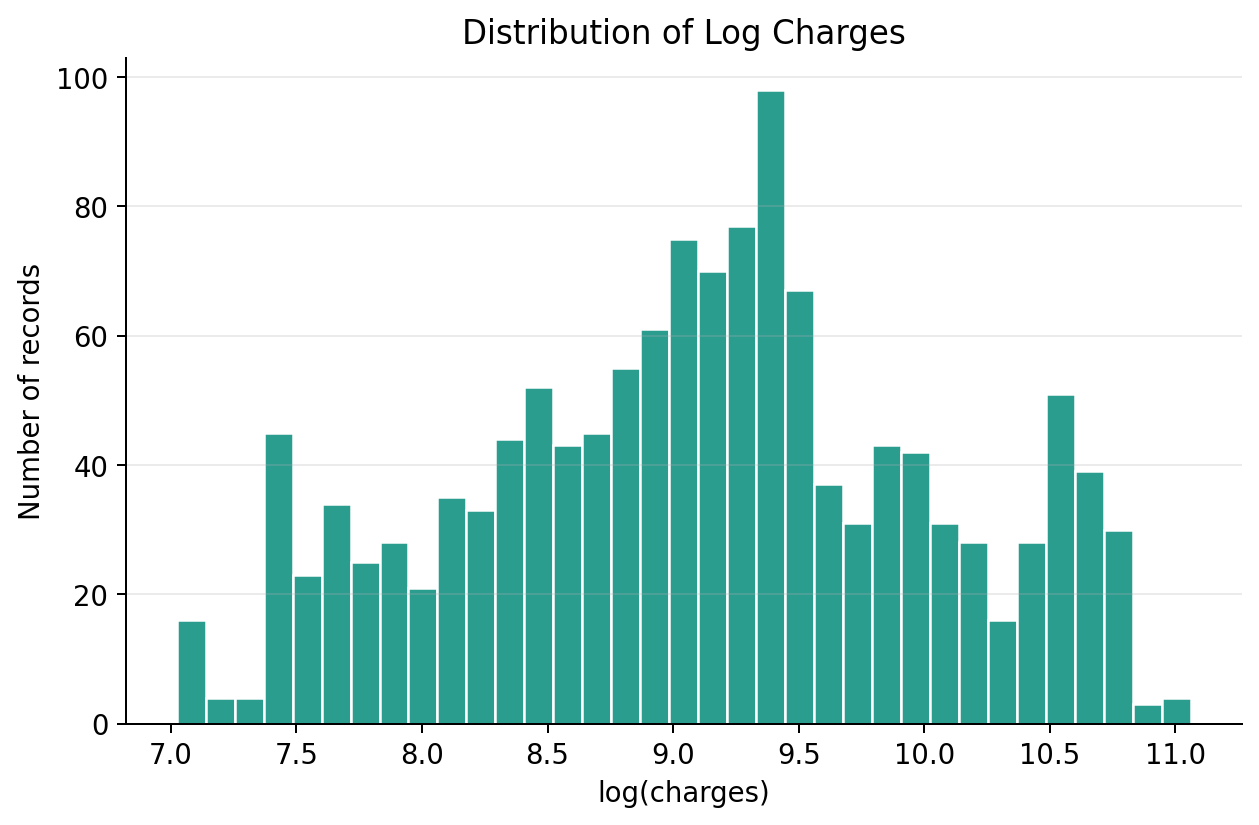
\includegraphics[width=0.82\textwidth]{log_charges_distribution.png}
    \caption{Distribution of log-transformed charges.}
    \label{fig:log-charges}
\end{figure}

The clearest visual separation appears in smoking status. As shown in Figure~\ref{fig:smoker-rate}, smokers have a much higher high-cost rate in this dataset. This is an association in the data, not proof of medical causation.

\begin{figure}[H]
    \centering
    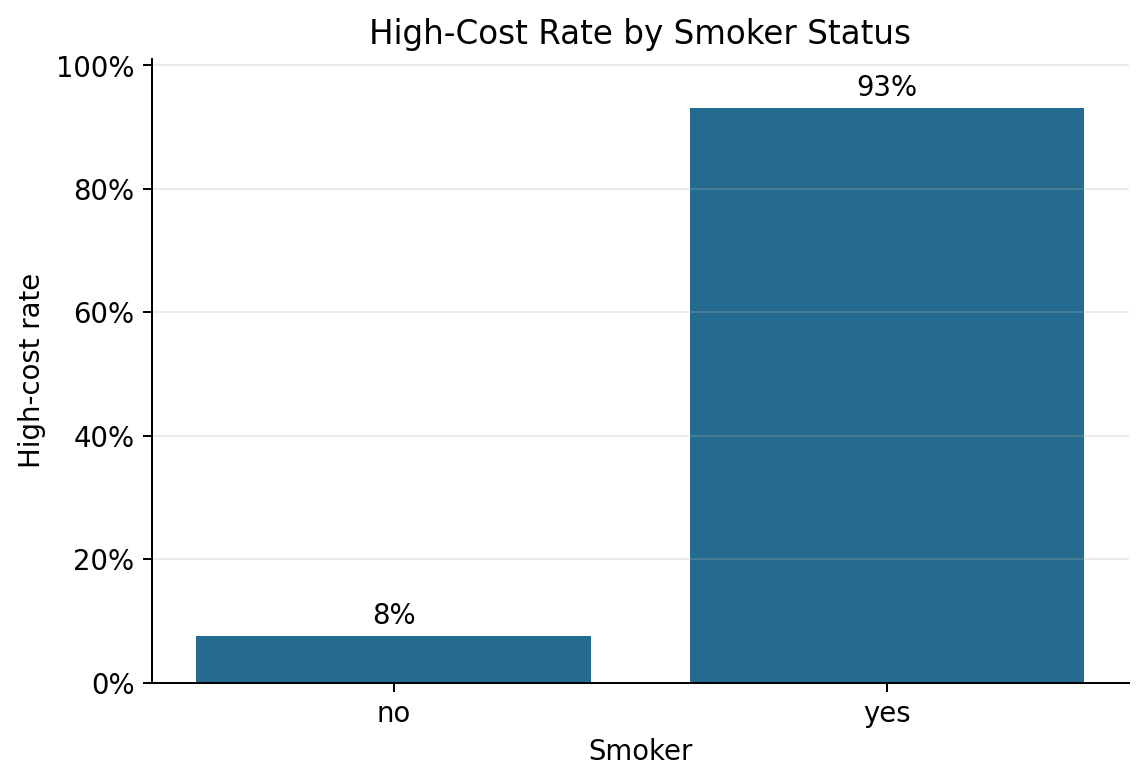
\includegraphics[width=0.74\textwidth]{high_cost_rate_by_smoker.png}
    \caption{High-cost rate by smoker status.}
    \label{fig:smoker-rate}
\end{figure}

BMI category and age group also show visible patterns. Figure~\ref{fig:bmi-rate} shows the high-cost rate by BMI category, while Figure~\ref{fig:age-rate} shows the high-cost rate by age group. These plots helped me decide which relationships were worth interpreting after modelling.

\begin{figure}[H]
    \centering
    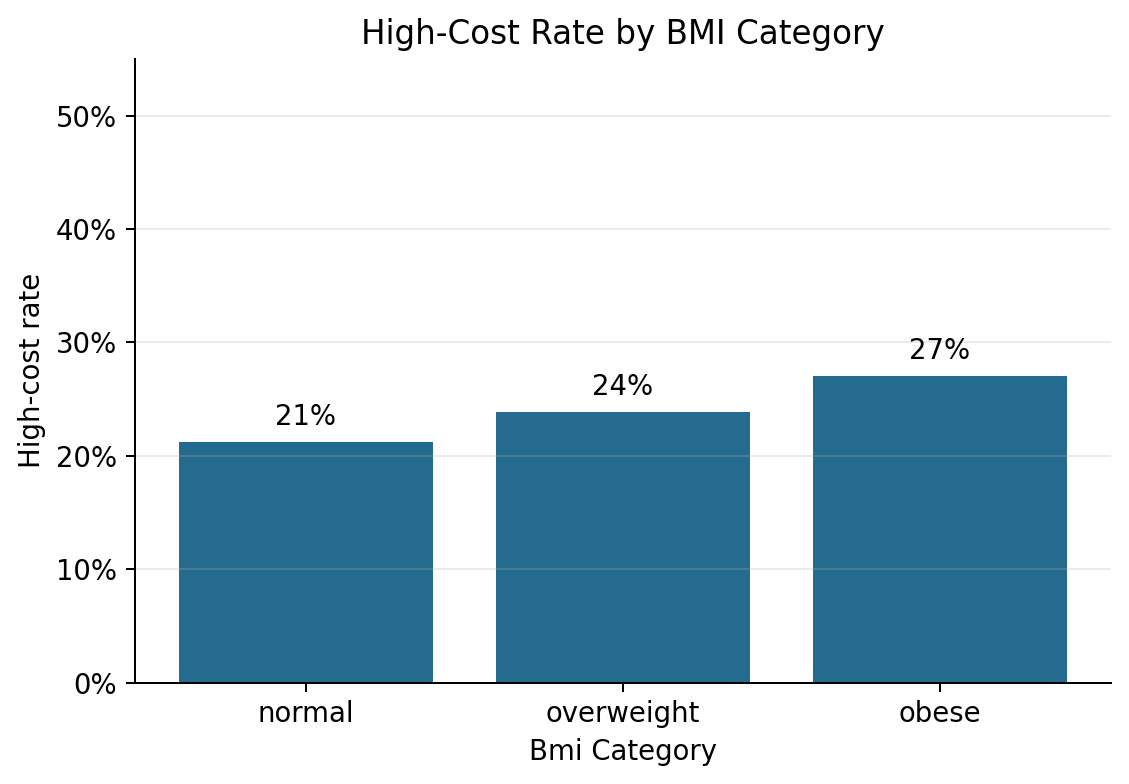
\includegraphics[width=0.74\textwidth]{high_cost_rate_by_bmi_category.png}
    \caption{High-cost rate by BMI category.}
    \label{fig:bmi-rate}
\end{figure}

\begin{figure}[H]
    \centering
    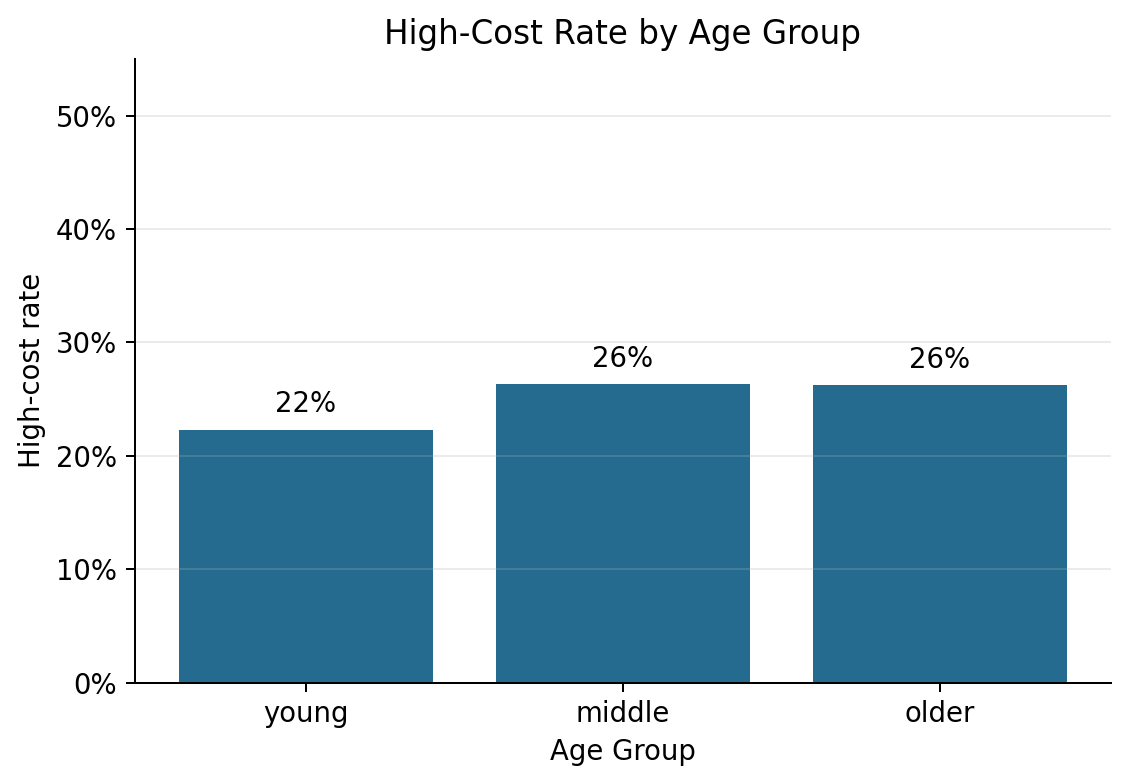
\includegraphics[width=0.74\textwidth]{high_cost_rate_by_age_group.png}
    \caption{High-cost rate by age group.}
    \label{fig:age-rate}
\end{figure}

The scatter plots in Figure~\ref{fig:age-scatter} and Figure~\ref{fig:bmi-scatter} show charges against age and BMI. They suggest that higher charges often appear at older ages and at higher BMI values, but the relationship is not perfectly linear.

\begin{figure}[H]
    \centering
    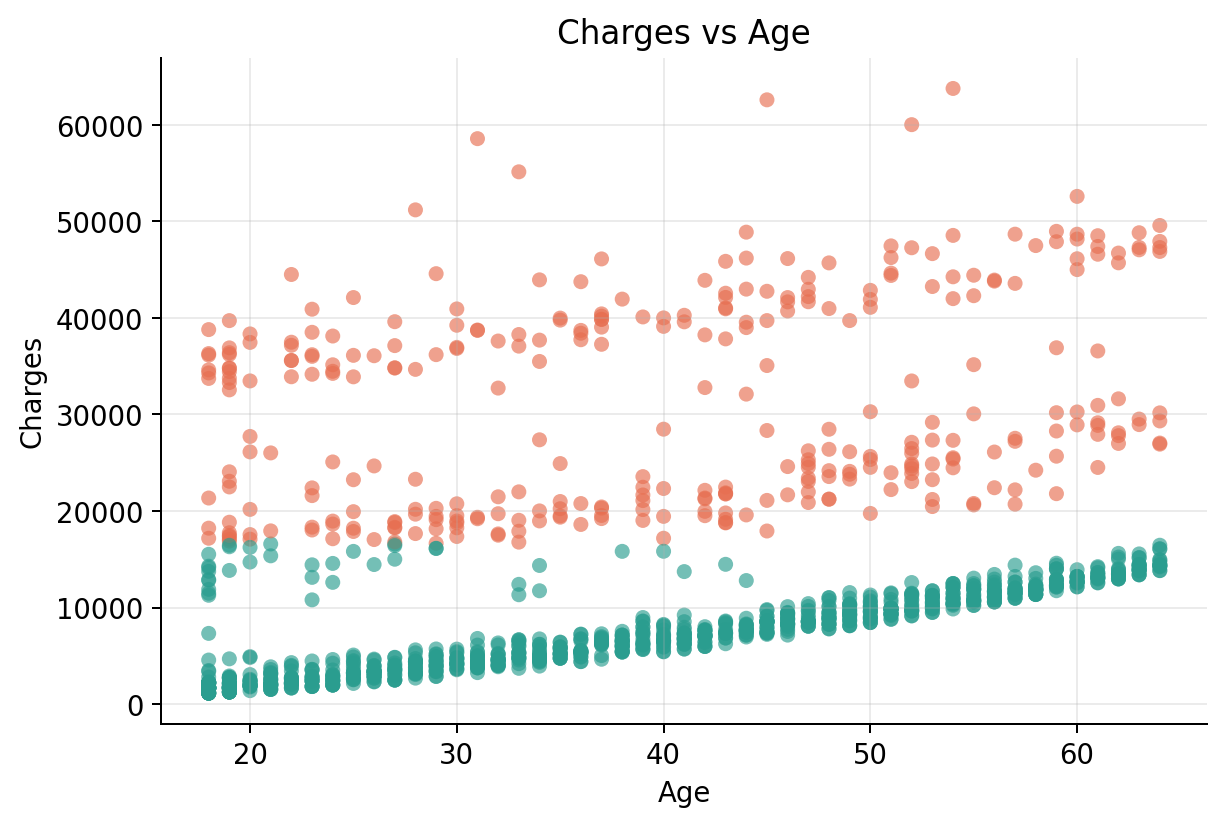
\includegraphics[width=0.78\textwidth]{charges_vs_age.png}
    \caption{Insurance charges plotted against age.}
    \label{fig:age-scatter}
\end{figure}

\begin{figure}[H]
    \centering
    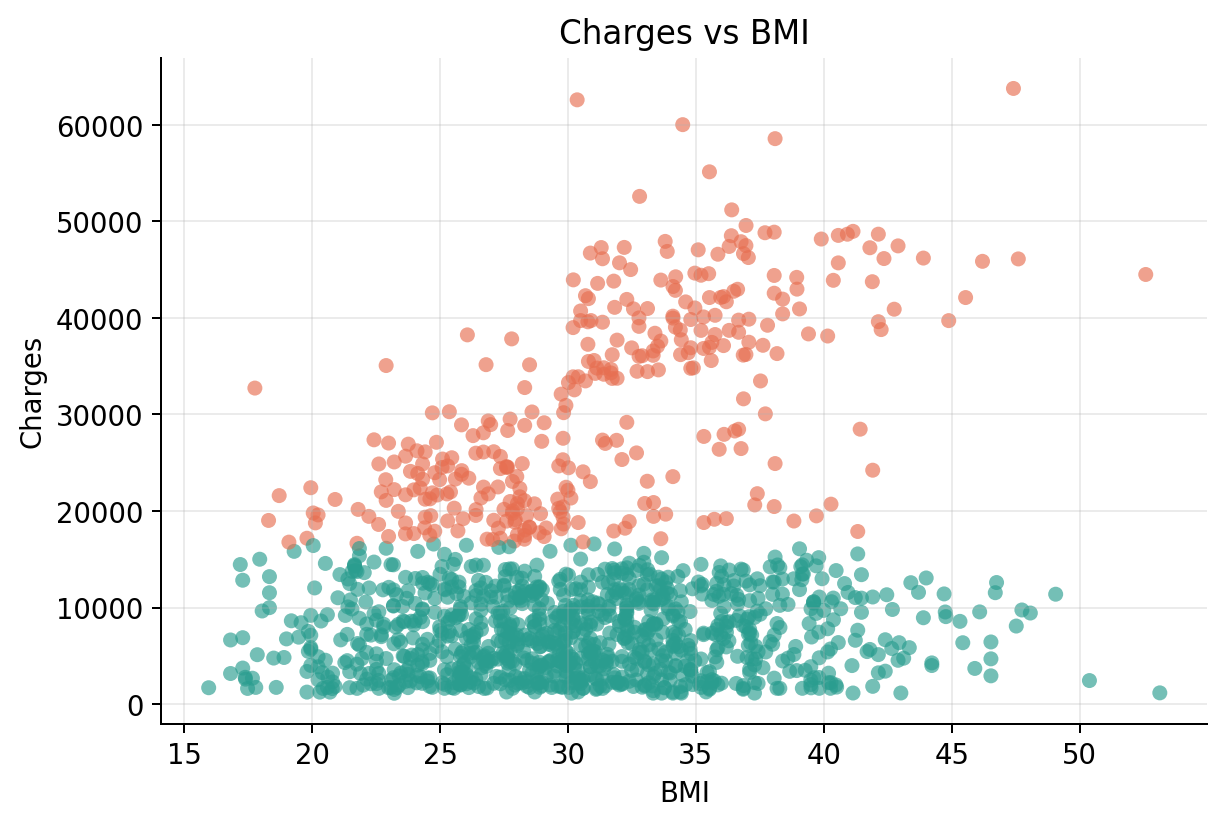
\includegraphics[width=0.78\textwidth]{charges_vs_bmi.png}
    \caption{Insurance charges plotted against BMI.}
    \label{fig:bmi-scatter}
\end{figure}

Figure~\ref{fig:corr} gives a numerical correlation matrix for the quantitative variables. Correlation measures linear association, not causation. This project studies statistical relationships in the dataset and does not prove medical causation.

\begin{figure}[H]
    \centering
    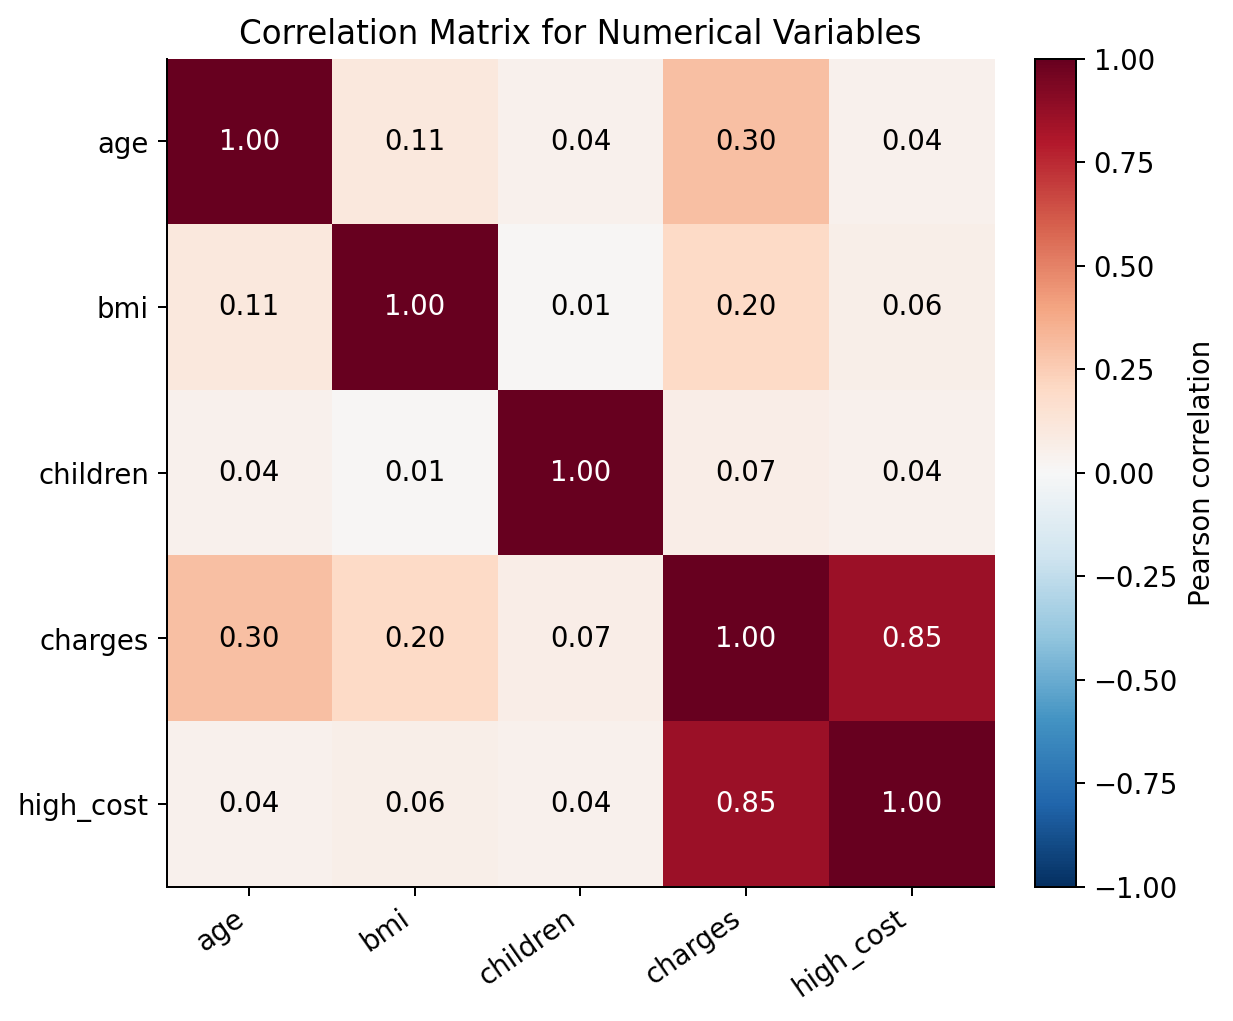
\includegraphics[width=0.72\textwidth]{correlation_matrix.png}
    \caption{Correlation matrix for numerical variables.}
    \label{fig:corr}
\end{figure}

\section{Logistic Regression}

Logistic regression models the probability \(p\) that a record belongs to the positive class, here \(\texttt{high\_cost}=1\). It uses the equation
\[
\log\left(\frac{p}{1-p}\right)
= \beta_0 + \beta_1 x_1 + \cdots + \beta_d x_d.
\]

The quantity
\[
\frac{p}{1-p}
\]
is the odds of the positive class. The logarithm of the odds is called the log-odds or logit. If
\[
z = \beta_0 + \beta_1 x_1 + \cdots + \beta_d x_d,
\]
then the predicted probability is obtained using the sigmoid function:
\[
p = \frac{1}{1+\exp(-z)}.
\]

The sigmoid function maps any real number into the interval \((0,1)\), which is why it can be used to produce probabilities. Very large positive values of \(z\) give probabilities close to 1, and very negative values give probabilities close to 0.

A coefficient \(\beta_j\) describes the change in log-odds for a one-unit increase in \(x_j\), holding other variables fixed. In odds form, a one-unit increase in \(x_j\) multiplies the odds by
\[
\exp(\beta_j).
\]

This interpretation is useful, but it is not causal. For example, a positive coefficient means the feature is associated with higher predicted odds in this fitted model. It does not prove that changing the feature would medically cause the charge category to change.

\section{Naive Bayes}

Naive Bayes is based on Bayes theorem:
\[
P(Y \mid X) = \frac{P(X \mid Y)P(Y)}{P(X)}.
\]

In this expression, \(P(Y)\) is the prior probability of the class before seeing the features, \(P(X)\) is the evidence, and \(P(Y \mid X)\) is the posterior probability after observing the features. The term \(P(X \mid Y)\) describes how likely the observed features are under a particular class.

The Naive Bayes simplification is the conditional independence assumption:
\[
P(x_1,\ldots,x_d \mid Y) = \prod_{j=1}^{d} P(x_j \mid Y).
\]

This assumes that, once the class \(Y\) is known, the features behave independently. In real healthcare-related data this assumption is probably too strong. Age, BMI, smoking status, and charges can be related in complicated ways. Still, Naive Bayes is useful here because the mathematics is transparent and the model gives a simple probabilistic baseline.

\section{Evaluation Metrics}

For both models, I used the same train/test split and the same metrics. Let \(TP\), \(TN\), \(FP\), and \(FN\) represent true positives, true negatives, false positives, and false negatives. The metrics are
\[
\text{Accuracy} = \frac{TP+TN}{TP+TN+FP+FN},
\]
\[
\text{Precision} = \frac{TP}{TP+FP},
\]
\[
\text{Recall} = \frac{TP}{TP+FN},
\]
and
\[
F1 = 2 \cdot \frac{\text{Precision}\cdot\text{Recall}}{\text{Precision}+\text{Recall}}.
\]

Accuracy measures overall correctness. Precision matters because it asks how reliable the high-cost predictions are. Recall matters because it asks how many of the actual high-cost records were found. Since the positive class is smaller than the negative class, accuracy alone could hide poor performance on the high-cost group.

Table~\ref{tab:model-comparison} compares the models on the test set. The two models perform very similarly here. I would not claim that one model is generally better from this single split.

\begin{table}[H]
\centering
\begin{tabular}{lrrrr}
\toprule
Model & Accuracy & Precision & Recall & F1-score \\
\midrule
Logistic Regression & 0.914 & 0.940 & 0.701 & 0.803 \\
Naive Bayes & 0.914 & 0.940 & 0.701 & 0.803 \\
\bottomrule
\end{tabular}
\caption{Test-set model comparison.}
\label{tab:model-comparison}
\end{table}

The confusion matrices in Figure~\ref{fig:cm-logistic} and Figure~\ref{fig:cm-nb} show the types of mistakes each model made. In this run, both models found many high-cost records but still missed some of them, which explains why recall is lower than precision.

\begin{figure}[H]
    \centering
    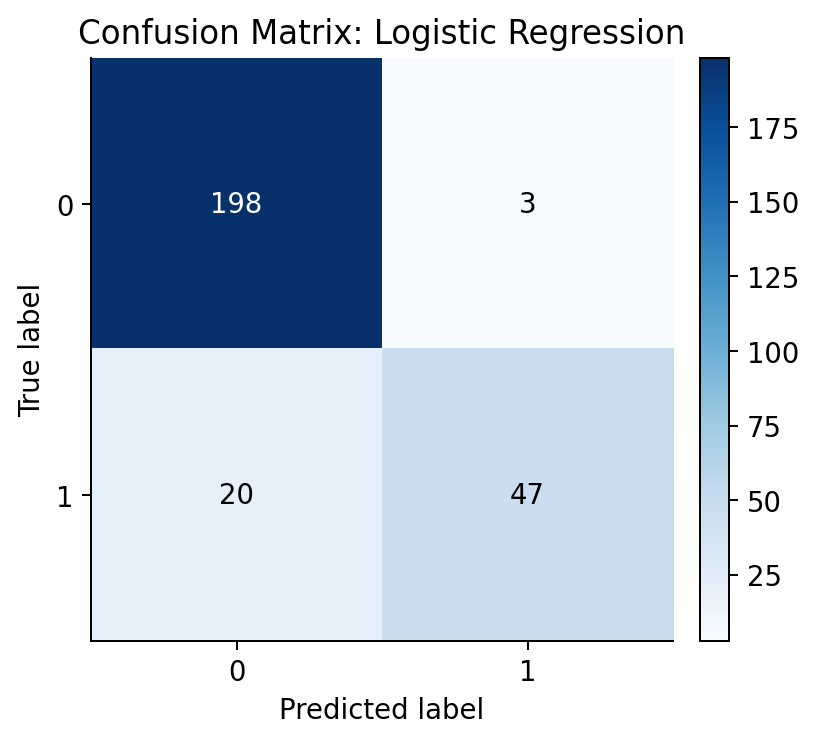
\includegraphics[width=0.56\textwidth]{confusion_matrix_logistic_regression.png}
    \caption{Confusion matrix for logistic regression.}
    \label{fig:cm-logistic}
\end{figure}

\begin{figure}[H]
    \centering
    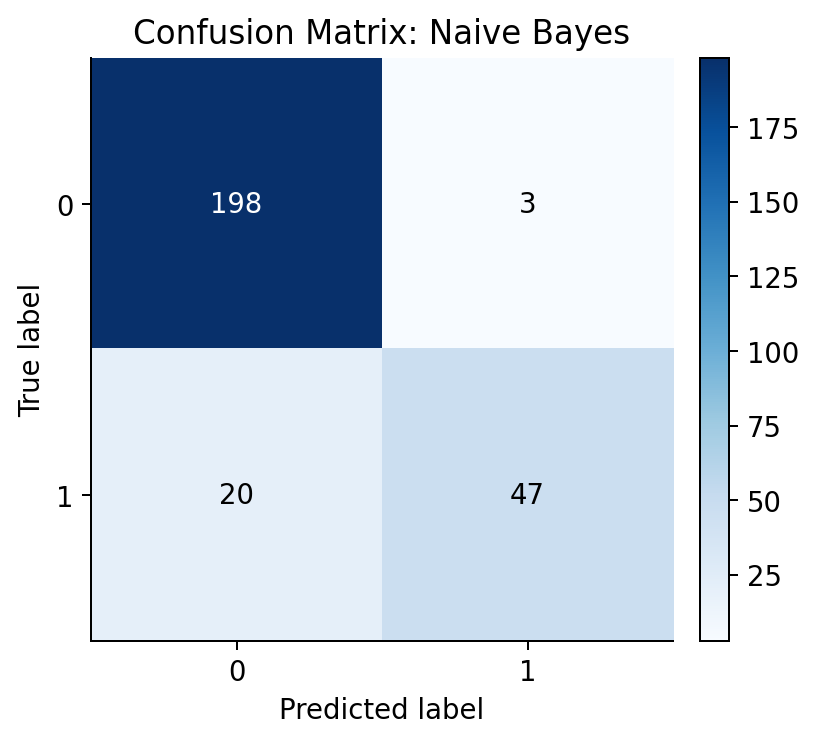
\includegraphics[width=0.56\textwidth]{confusion_matrix_naive_bayes.png}
    \caption{Confusion matrix for Naive Bayes.}
    \label{fig:cm-nb}
\end{figure}

\section{Main Observations}

One interesting observation was that smoking status separated the high-cost and not-high-cost classes quite strongly. I also noticed visible relationships involving age and BMI. Logistic regression was easier for me to interpret through coefficients and odds multipliers. Naive Bayes was useful for practising Bayes theorem and conditional probability.

The main result is modest: two simple models performed similarly on this dataset. This is enough for the goal of the project, which is to demonstrate a careful and interpretable workflow rather than to claim clinical usefulness.

\section{Limitations and Future Work}

The most important limitation is that the target is based on insurance charges, not medical diagnosis or medical risk. The threshold is also arbitrary and chosen for educational reasons. The dataset is small and simplified, and the analysis uses one train/test split.

Future improvements could include cross-validation, trying alternative high-cost thresholds, checking probability calibration, and adding a short fairness discussion. Even with those improvements, the project would still need careful wording: prediction is not causation, and correlation is not clinical evidence.

\section{Conclusion}

This project gave me a practical way to connect coding with the mathematics behind classification. Logistic regression helped me understand probabilities, odds, log-odds, and coefficients. Naive Bayes helped me practise Bayes theorem and conditional independence. The evaluation step showed why precision and recall are useful when the target is imbalanced.

This project studies statistical relationships in the dataset and does not prove medical causation.

\begin{thebibliography}{9}

\bibitem{hunter2007}
J. D. Hunter.
Matplotlib: A 2D graphics environment.
\textit{Computing in Science \& Engineering}, 9(3):90--95, 2007.

\bibitem{mckinney2010}
W. McKinney.
Data structures for statistical computing in Python.
\textit{Proceedings of the 9th Python in Science Conference}, pages 56--61, 2010.

\bibitem{pedregosa2011}
F. Pedregosa et al.
Scikit-learn: Machine Learning in Python.
\textit{Journal of Machine Learning Research}, 12:2825--2830, 2011.

\end{thebibliography}

\end{document}
